\documentclass[a4paper,UKenglish]{dagrep}

\usepackage[utf8]{inputenc}
\usepackage{microtype}

\bibliographystyle{plain}

\iffalse
\usepackage{draftwatermark} % option '[nostamp]' to ignore watermark
\SetWatermarkFontSize{5cm}
\SetWatermarkScale{0.5}
\SetWatermarkLightness{0.8}
\SetWatermarkColor[rgb]{0.95,0.4,0.1}
\SetWatermarkText{\shortstack[l]{\vspace*{3cm}\ \textsf{DRAFT 2016-09-14}}}
\fi

\subject{Report from Dagstuhl Seminar 16251}
\title{Information-centric Networking and Security}
\titlerunning{16251 -- Information-centric Networking and Security}

\author[1]{Edith Ngai}
\author[2]{Börje Ohlman}
\author[3]{Gene Tsudik}
\author[4]{Ersin Uzun}
\author[5]{Christopher A. Wood}
\authorrunning{Edith Ngai, Börje Ohlman, Gene Tsudik, Ersin Uzun, and Christopher A. Wood}
\affil[1]{Uppsala University, SE, \texttt{edith.ngai@it.uu.se}}
\affil[2]{Ericsson Research - Stockholm, SE, \texttt{borje.ohlman@ericsson.com}}
\affil[3]{University of California - Irvine, US, \texttt{gts@ics.uci.edu}}
\affil[4]{Xerox PARC - Palo Alto, US, \texttt{ersin.uzun@acm.org}}
\affil[5]{University of California - Irvine, US, \texttt{woodc1@uci.edu}}



\seminarnumber{16251}
\semdata{June 19--22, 2016 -- \href{http://www.dagstuhl.de/16251}{http://www.dagstuhl.de/16251}}

\volumeinfo%(easychair interface)
  {Edith Ngai, Börje Ohlman, Gene Tsudik, and Ersin Uzun}%editor names
  {4}%number of editors
  {Information-centric Networking and Security}%seminar title
  {6}%volume
  {06}%issue
  {1}%starting page number
\DOI{10.4230/DagRep.6.6.1}%(DagRep.<volume no>.<issue no>.<firstpage>)

\begin{document}

\maketitle

\begin{abstract}
In recent years, Information-centric Networking (ICN) has received much attention from both academic and industry participants. ICN offers a data-centric means of inter-networking that is radically different from today's host-based IP networks. Security and privacy issues in ICN have become increasingly important as ICN technology gradually matures and nears real-world deployment. As is well known, in today's Internet, security and privacy features were originally not present and had to be incrementally and individually retrofitted (with varying success) over the last 35 years. In contrast, since ICN-based architectures (e.g., NDN, CCNx, etc.) are still evolving, it is both timely and important to explore ICN security and privacy issues as well as devise and assess possible mitigation techniques. 

This report documents the program and outcomes of the Dagstuhl Seminar 16251 ``Information-centric Networking and Security.'' The goal was to bring together researchers with different areas of expertise relevant to ICN to discuss and grapple with some of the large outstanding security and privacy problems particular to ICN-based architectures. The represented areas of expertise included networking, security, privacy, software engineering, and formal methods, among others. Through generalized presentations and focused working groups, the attendees attempted to unveil emerging problems, highlight outstanding issues relevant to security and privacy, and work towards solutions in ICN-based architectures. 
\end{abstract}

% Executive Summary %%%%%%%%%%%%%%%%%%%%%%%%%%%%%%%%%%%%%%%%%%%%%%%%%%%%%%%%%%%%%%%%%%%%%%%%%%%%%%%%

\section{Executive Summary}

\summaryauthor[Christopher A. Wood]{}
\license

The Dagstuhl seminar 16251 "Information-centric Networking and Security" was a short workshop held from June 19-21, 2016. The goal was to bring together researchers with different areas of expertise relevant to ICN to discuss and grapple with some outstanding security and privacy problems particular to ICN-based architectures. These problems have become increasingly important as ICN technology gradually matures and nears real-world deployment. 

The threat models for ICN are distinct from IP. Differentiating factors between the two include new application design patterns, unique trust models and management, and a strong emphasis on object-based security instead of channel-based security. Therefore, it is both timely and important to explore ICN security and privacy issues as well as devise and assess possible mitigation techniques. This was the general purpose of the Dagstuhl seminar. To that end, the attendees focused on the following issues in particular:
%
\begin{itemize}
\item What are the relevant threat models with which ICN must be concerned? How are they different from those in IP-based networks?
\item To what extent is trust management a solved problem in ICN? Have we adequately identified the core elements of a trust model, e.g., with NDN trust schemas?
\item How practical and realistic is object-based security when framed in the context of accepted privacy measures used in IP-based networks?
\item Are there new types of cryptographic schemes or primitives ICN architectures should be using or following that will enable (a) more efficient or secure packet processing or (b) an improved security architecture?
\end{itemize}
%
The seminar satisfied many of these questions and fueled discussions for those remaining. To begin, all participants briefly self-introduced themselves. Afterwards, select participants contributed talks on various topics of interests, ranging from trust management and identity to an exploration of privacy and anonymity. Between these primary discussions, the group partitioned itself into various working groups to focus more intensely on a select topic of interest to the subgroup. Example topics included routing on encrypted names, ICN and IoT, non-privacy-centric aspects of ICN security, and trust and identity in ICN. Following these working groups, a representative from each would present the findings to the group. (These are documented in the remainder of this report.)

The major takeaways from the seminar were as follows. First, the ICN community still does not have a clear answer for how namespace and identity management will be handled. While trust management in ICN can be distributed without a PKI, it seems difficult to break away from this model for namespace management and arbitration. This has strong implications on how names are propagated in the routing fabric. Can any producer application advertise any name they want, anywhere in the network? If not, how will advertisements be constrained or limited?

Second, given that ICN focuses on object security, the need for and use of transport protocols that provide forward secrecy should be deferred to an upper layer in the stack. Attendees found that while most ICN-based architectures do not preclude forward secrecy, it should not be a requirement for the core network protocol. 

Third, there is still deep uncertainty about whether ICN should embrace a content locator and identifier split. Names in architectures such as NDN and CCN serve as both a locator and identifier of data, though extensions do exist to permit explicit locators (e.g., through the use of NDN LINK objects). This distinction is necessary under the common understanding that routing should concern itself with topological names; Finding data through non-topological names should not be in the data plane as part of the global routing space. However, if we revert to a distinction between topological locators and identifiers, then features characteristic of ICN become much more limited. One facet that is certainly unique to ICN is how software is written. Specifically, we have the opportunity to move beyond the mental model of a fixed address space and re-design existing network stacks and APIs. 

Fourth, privacy seems difficult to achieve without major architectural changes to many existing ICN-based systems. In particular, since data names reveal a great deal of information to the passive eavesdropper, privacy here would imply that names and payloads have no correlation. However, achieving this particular goal seems infeasible without the presence of an upper-layer service akin to one that would resolve non-topological identifiers to topological names. 

Lastly, it is clear that ICN-based architectures should not yet be exploring the use of esoteric cryptographic algorithms in the network. Computationally bounded and ``boring'' cryptographic primitives, such as digital signatures, hash functions, etc., should be the extent of per-packet cryptographic processing done by routers. Anything more could unnecessarily induce computational Denial-of-Service attacks that could render the entire infrastructure ineffective. However, architecture designs should not restrict themselves to specific algorithms. They should allow new and improved algorithms to be used as their need becomes apparent. This could be useful if, for example, post-quantum digital signature schemes become necessary for the longevity of content authenticators. 

We thank Schloss Dagstuhl for the environment necessary to galvanize members of the ICN community to address these difficult problems. Much progress was had over the course of the seminar and since its completion, and this is primarily because of the ease of face-to-face collaboration and interaction held at Dagstuhl.

\tableofcontents

% Overview of Talks %%%%%%%%%%%%%%%%%%%%%%%%%%%%%%%%%%%%%%%%%%%%%%%%%%%%%%%%%%%%%%%%%%%%%%%%%%%%%%%%

\section{Overview of Talks}

\abstracttitle{Threat Models for ICN}
\abstractauthor[Ersin Uzun]{Ersin Uzun (Xerox PARC - Palo Alto, US)}
\license

IP-based networks helped to create today's world of content but was not designed for it. ICN attempts to move away from: (a) the communication model that is all about hosts and a point-to-point conversation between them, (b) the host-based central abstraction in the network, and (c) security problems of the current IP-based Internet architecture. The ICN emphasis on object security instead channel security is one step towards this transition. To quantify the degree by which security is improved, a thread model is needed. These threat models must be tailored toward the particular design challenge, such as infrastructure protection, user-friendly key distribution and trust management and enforcement, and content protection and access control. We discuss some necessary elements of threat models for these scenarios and suggest a strategy to use them in the ICN security design process.

\abstracttitle{Cryptographic Algorithms and Security Protocols for ICN}
\abstractauthor[Christopher A. Wood]{Christopher A. Wood (University of California - Irvine, US)}
\license

We present a survey of old and new cryptographic algorithms and security protocols with relevance to ICN packet processing, routing, and object security. Select topics include integrity and authenticity, privacy, and availability, as these are the main security goals of ICN-based architectures. The objective is to stimulate useful discussions about the characteristics and implementation of security services and properties that future ICN-based architectures might provide.

\abstracttitle{Violating Consumer Anonymity: Geo-locating Nodes in Named Data Networking}
\abstractauthor[Mauro Conti]{Mauro Conti (University of Padova, IT)}
\license

Talking about ICN privacy, we should not focus only on ``what'' (i.e., the content of a message) and ``who'' (i.e., the sender, or the receiver, of a message): we should also be worried about protecting "where", meaning the geographical position (or just the position within a network topology) where the message is originated from, or destined to. In fact (as shown in the ACNS '15 paper by Compagno et al. [1]), ICN caching and interest-collapse mechanisms make ICN itself inherently vulnerable to the possibility for an adversary to locate consumers.
Interestingly, an approach similar to the one to violate consumer (location) privacy, might be used also to detect eavesdropper.
Discussion questions included:
\begin{itemize}
\item Exactly what routing information is made available to routing-aware adversaries, and how useful is it to run attacks?
\item By observing past traffic, can one infer where interests will be routed in the network?
\item What capabilities does the adversary possess?
\item How does this compare to similar attacks in IP?
\end{itemize}

\begin{thebibliography}{0}
[1] Alberto Compagno, Mauro Conti, Paolo Gasti, Luigi Vincenzo Mancini, Gene Tsudik:
Violating Consumer Anonymity: Geo-Locating Nodes in Named Data Networking. ACNS 2015: 243-262.
\end{thebibliography}

%%%%% XXXX: here

\abstracttitle{ABE in ICN}
\abstractauthor[Ashish Gehani]{Ashish Gehani (SRI - Menlo Park, US)}
\license

The ENCODERS information-centric networking system was designed for publish-subscribe applications running over a mobile ad hoc network. It uses multi-authority attribute-based encryption to allow content access to be scoped to selected nodes in the system. Since the system is completely decentralized, peers serve as brokers that match content from publishers with interests expressed by subscribers. In order to perform such a match, an intermediate node must be authorized to see both the relevant content tags and  subscriber interests. All of this has been described in a previous publication [1].

The talk described the following unpublished observation. The access control policies that applied to the metadata (content tags and subscriber interests) effectively creates reachability constraints that are independent from the one defined by the routing protocols. (This is because the access control defines which brokers can match and therefore route traffic.) Consequently, this security-routing interaction must be treated carefully during policy definition. We examined this empirically for a number of routing and access control policies.

\begin{thebibliography}{0}
[1] Mariana Raykova, Hasnain Lakhani, Hasanat Kazmi, and Ashish Gehani, Decentralized Authorization and Privacy-Enhanced Routing for Information-Centric Networks, 31st Annual Computer Security Applications Conference (ACSAC), 2015.
\end{thebibliography}

\abstracttitle{PROJECT ORIGIN: A peer-to-peer object store for CCN}
\abstractauthor[Marc Mosko]{Marc Mosko (Xerox PARC - Palo Alto, US)}
\license

Project Origin is a bittorrent-like system for CCNx that uses concepts of nameless objects and custodian routing to achieve a scalable, secure content distribution system. In this talk we present the initial design of Project Origin in the context of CCNx.

\abstracttitle{In-Network Processing and Related Laws}
\abstractauthor[Tohru Asami]{Tohru Asami (University of Tokyo, JP)}
\license

The history of the Internet is the one to adapt the existing law system
to our new business paradigms. The level of in-network processing has
been expanded as (1) Routing, (2) Forwarding, (3) Packet replication,
(4) Merging/Splitting packets, (5) Quality of Control, (6) Caching, (7)
Switching with moderate packet inspection (NAT),(8) SDN/NFV, (9)
Extended data processing using in-network data object. We all have been
crossing together on the red light since every new technology has
violated the existing laws to some extent.
The first conflict was Cache/Replication against Copyright law. Before
the revision of the Copyright Act in 2009, the followings violated our
copyright laws in Japan but the government overlooked these services: (1)
Internet search service (i.e., Google), (2) backup of the customers' e-mail
folders by Internet service providers, (3) packet replications in IP
routers, and (4) P2P service. Accidentally, Isamu Kaneko, the developer
of Winny (a P2P program), was arrested on suspicion of abetting
copyright law violation in 2004. During the course of this court battle,
in 2009, the use of cache was legally admitted in Japan on providing
communication services to the extent deemed necessary in order to carry
out the transmission efficiently.
We all are still crossing together on the red light in the problem of
“Secrecy of Correspondence vs Packet Header Processing.” This case is
more severe since this time is the conflict against our fundamental
human rights. Thus our constitution or laws prohibit knowing, disclosing
and using the secrecy of correspondence without ``permission.''
According to the postal businesses, main theorists in law have been
requiring the whole secrecy of correspondence or the secrecy for both
the header (envelope) and the payload (letter paper), while minor
theorists requiring only the secrecy of payload. However, in the
practical postal services, envelopes have been intensively used to
classify mails as ordinary mails (default), registered mails,
confidential mail, contents-certified mail, etc. The mails rather than
ordinary mails are identified by the ``explicit requirement of a sender.''
This is the important tradition to remember.
As for secrecy of correspondence operated by the Internet, routers use
packet headers without permission from the sender. The following
in-network processing may violate Secrecy of Correspondence: 1)IP packet
forwarding, 2)Software Defined Network (SDN) detecting a traffic flow
based on IP addresses and port numbers to control, 3) ICN Cache ranking
by names for prioritization, etc. Thus several exceptions have been
defined by individual laws.
Now we are facing at the age that most of the traffic is carried by
HTTPS. It is highly possible that Deep Packet Inspection (DPI) of
SSL/TLS packets violates Secrecy of Correspondence since the targeted
packets declare their secrecy intention by encryption, even if DPI
is technically possible. In fact, although DPI is one of the
technologies to perform a behavioral targeting advertising, it is not
carried out in many countries because of the reason that it may violate
Secrecy of Correspondence and may be illegal.
As for the policy of Secrecy of Correspondence/Privacy, two policies
have been discussed: All-or-nothing Policy and Policy of Controllability.
Most researchers as well as the discussions in this seminar are fond
of the former secrecy, but I’m afraid that the former will not expand
the network business. The latter requires that owner can control his/her
information at hand. This is what postal services have been based on as
well as our fruitful future in-network processing business. According to
this policy, the sender's intention on secrecy or preference of
in-network processing should be declared in the optional ``header'' field
of the sending/receiving ICN packet in an opt-in fashion as the content
owner's contract with the network provider. The default is, of course,
that everything other than content name is secret (so as to EU Data
Protection Directive/Regulation). Since ICN routers left less
communication logs than the conventional IP routers, they will be
welcomed from the view point of Secrecy of Correspondence/Privacy. This
is the advantage of ICN against IP in the age of secure communications,
and we should promote ICN from this perspective.
In conclusion, ICN packet header should have enough information for
future in-network processing. From the point of secrecy of
correspondence/Privacy, ICN header should reflect the intent of
packet sender on secrecy and privacy by its optional header. Otherwise,
there will be a large risk that ICN in-network processing is regarded as
violating privacy and secrecy of correspondence.

\begin{thebibliography}{0}
[1] FireEye SSL Intercept Appliance -- Expose Attacks Hiding in SSL Traffic. Available online at: \url{https://www.fireeye.com/content/dam/fireeye-www/global/en/products/pdfs/ds-ssl-intercept.pdf}. Accessed on 9/15/2016.
\end{thebibliography}

%\abstracttitle{Quantum Computing and Cryptography}
%\abstractauthor[Ersin Uzun]{Ersin Uzun (Xerox PARC - Palo Alto, US)}
%\license
%
%A summary of the advancements and implications of quantum computing and cryptography is discussed. The goal is to give the audience context when discussing the relevance of quantum computing and the necessity of post-quantum cryptography.

%\newpage

% Working groups %%%%%%%%%%%%%%%%%%%%%%%%%%%%%%%%%%%%%%%%%%%%%%%%%%%%%%%%%%%%%%%%%%%%%%%%%%%%%%%%%%%

\section{Working groups}

\abstracttitle{Names and Locators}
\abstractauthor[Marc Mosko]{Marc Mosko (Xerox PARC - Palo Alto, US)}
\license

The CCNxTorrent working group discussed locators and fetching data with non-topological names (or even topological names that are cached off-path). Routing should, it seems, only concern itself with topological names or addresses.  Finding data (objects) with non-topological names should not be done in the data plane.  It should be done via a service.

In CCNx, the service could resolve a named root manifest to then resolve locator names by hash.
In NDN, it resolves the link routing hints to allow off-path interest forwarding. In TagNet,
there is a distinction between Locator names and Descriptor names. Locator names have a
strong binding between their name and a point of attachment. Descriptor (hash) names, on the
other hand, are free-form and could be present anywhere.  One resolves a tag query (of either
type) to a topological locator and then does data transfer on that locator.

This lead to a discussion on locator and identifier split.  Should CCNx embrace this, or continue on with its mixed use of the name? For example, if there is a clear locator field and then a clear identifier tuple \{name, [keyed restriction], [hash restriction]\}, one would get full matching expressivity with the functionality of nameless object locators.  A similar approach could be done in NDN, though with a different tuple.  There was no consensus on this idea, though it is worth exploring.

There was some discussion on the benefit of ICN if one still needs to do an external name to address lookup.  Why bother if one still needs an IP- or DNS-like function?  One partial answer is that in the non-global routing space (i.e., data center, maybe IoT, some internal applications), one could inject all names into the internal routing protocol and realize the full benefit of application-specific names.  Another argument is that it improves how one writes software to not have to deal with IP addresses and host-based networking. One could also see benefits from a re-thought network stack beyond sockets.

\abstracttitle{ICN and IoT}
\abstractauthor[Edith Ngai]{Edith Ngai (Uppsala University, SE)}
\license

The Internet of Things (IoT) is connecting billions of smart devices (e.g. sensors) and is growing very fast. We expect more than 1 million networked ``things'' per square kilometer in 2030. In this group, we tried to explore how much data density we can afford
and how we communicate with the ``things'' (say, directly to the sensors, or indirectly through the cloud or gateways). We discussed the potential of implementing ICN for the IoT. For instance, the ICN routers connecting to sensors can cache sensor data to improve the performance of data dissemination. Users can obtain data directly from the sensors and the ICN routers, without going through the cloud. There are several security concerns:

\begin{itemize}
\item How are sensors securely configured at the time of initialization?
\item How can software updates be performed securely?
\item How can we handle ICN mobility for IoT? For example, each sensor may have unique publisher identity. How do mobility and naming affect the scalability of routing?
\end{itemize}

We discussed the potentials and concerns of caching data at the sensors:

\begin{itemize}
\item Sensors are resource limited devices. However, memory resources may increase and the price will go down.
\item It is advantageous to retrieve data directly from the sensors in some use cases (e.g., to control home lighting without going through the cloud).
\item When using cryptography on sensors, the encryption time could be long and cause a delay in data retrieval.
\item Sensors have to be always on to listen to the interests, which may consume a lot of energy. Scheduling or adaptive duty cycles might be considered to mitigate this.
\end{itemize}

Our summary and future plan is as follows. First, we plan to come up with sample IoT use cases, which allow us to understand more about the security needs and communication patterns in ICN for IoT. Second, we will aim at answering the following questions:

\begin{itemize}
\item How does IoT benefit from ICN?
\item How to configure sensors at bootstrapping?
\item Explore the cost of providing security for IoT data
\end{itemize}

\abstracttitle{Security, Not Privacy}
\abstractauthor[Craig Partridge and Ghassan Karame]{Craig Partridge (BBN Technologies - Cambridge, US) and Ghassan Karame (NEC Laboratories Europe - Heidelberg, DE)}
\license

The ``No Privacy'' security working group sought to answer the following question: is an ICN security architecture easier to devise if the designs fundamentally make privacy hard to achieve? In particular, the group discussed:

\begin{itemize}
\item What ICN entities (content consumers, hosts, routers, content creators) need identities?
\item What entities can simply operate with a public/private key pair but no formal name?
\item Does splitting routing out as an application help?
\item Do interests need to be authenticated at each router?
\end{itemize}

The group achieved a simple security model. Members of the group hope to write up the result as a short paper.

\abstracttitle{Trust and Identity in ICN}
\abstractauthor[Jan Seedorf, Kenneth L. Calvert, and Christopher A. Wood]{Jan Seedorf (NEC Laboratories Europe - Heidelberg, DE \& Hochschule f\"ur Technik - Stuttgart, DE), Kenneth L. Calvert (University of Kentucky - Lexington, US), and Christopher A. Wood (University of California - Irvine, US)}
\license

In an ideal ICN architecture, applications should be able to express their trust preferences or policies and let the "middleware" enforce them. This raises two important questions: (1) what is the minimum set of policies that can be factored out of all trust models, and (2) what is the middleware that does this enforcement? The trust schemas pioneered by the NDN architecture [1] are exemplary of the core rules that might encompass a trust model. They specify what keys are allowed to sign what data. Since both keys and data are named resources in NDN and other ICN architectures, this means that a schema is, at its core, a simple name-to-name mapping that allows for arbitrary hierarchical trust models. It remains to be seen if other non-hierarchical trust models will be applicable to ICN.

To address the second question, we had to agree upon what the network is responsible for enforcing.
First and foremost, network layer ``trust enforcement'' should not prohibit or prevent other application-layer trust models. This means that the network functionality must be simpler than that which is supported by the middleware. Currently, this is comprised of digital signature and content object hash verification. Behaviors such as certificate chain resolution or key retrieval should not be part of the core network functionality. This means that in the general "network," routers are only responsible for single signature or hash verification. All other network nodes (e.g., consumers and producers) contain the middleware responsible for handling the remaining trust enforcement steps.

After addressing trust, we turned to identity and discussed the following major questions:
%
\begin{itemize}
\item How are names registered and managed in ICN?
\item How can names possibly be location agnostic? Is there always a discovery or locator service?
\end{itemize}
%
Namespace ownership is intrinsically tied to identity. Thus, namespace advertisements under different namespaces or in different networks must be authenticated with respect to the claimed owner's identity. In this context, an identity is a public and private key pair. We struggled with questions about namespace scale and the practicality of a global namespace. Questions such as, "how do NATs work in a global namespace," drove the discussion. No consensus or common understanding was reached.

\begin{thebibliography}{0}
Yingdi Yu, kc claffy, Alexander Afanasyev, Van Jacobson, David Clark, and Lixia Zhang. "Schematizing trust in named data networking." Proceedings of the 2nd International Conference on Information-Centric Networking. ACM, 2015.
\end{thebibliography}

\abstracttitle{Routing on Encrypted Names}
\abstractauthor[Christopher A. Wood, Edith Ngai, Jan Seedorf, and Matthias W\"ahlisch]{Christopher A. Wood (University of California - Irvine, US), Edith Ngai (Uppsala University, SE), Jan Seedorf (NEC Laboratories Europe - Heidelberg, DE \& Hochschule f\"ur Technik - Stuttgart, DE), and Matthias W\"ahlisch (FU Berlin, DE)}
\license

This group started with a discussion about routing on encrypted names but ended up being a discussion about name privacy and the necessary conditions for it to be possible in different ICN architectures. In this context, we defined name privacy to be a property where a so-called "network name," i.e., the name encoded in a packet, has no correlation or connection with the referenced content object. Specifically, name privacy means that a network name reveals nothing about the data inside the content object. Names should reveal no more than what is currently revealed by an IP address and port. After settling on this definition, we laid out our assumptions, including:

\begin{itemize}
\item There is no name discovery process or search engine.
\item Content may be requested by an identifier (ID) such as its cryptographic hash digest. Moreover, revealing the content ID does not compromise privacy.
\item Consumers know the public key of the producer to which they want to communicate.
\item Network names have an implicit routable prefix and application-specific suffix. By default, consumers do not know the locator and identifier split in a name.
\item Requests may specify the ID of a signature verification key or the expected content.
\end{itemize}

There are fundamentally two ways to request content: (1) with and (2) without a content ID. In case (1), a request name needs to only contain a routable prefix that will bring the request to some cache or producer which can return the corresponding content. These locators can be completely separate from the desired content and, therefore, this approach can satisfy our name privacy goal. However, without implicit knowledge about the locator for some desired content, an upper-layer service is necessary to obtain said information.

In case (2), the application-specific suffix of a name must not reveal anything about the data. To achieve this, it must be encrypted. Name encryption introduces a number of other questions, such as how to obtain the routable prefix, what key to use for encryption, and how to ``protect'' the result. For the base case, assume that the routable prefix is known and that the producer public key is used for name suffix encryption. If the resultant content payload is not encrypted then one may be able to infer the name from its contents. Therefore, the content response itself must also be encrypted. This requires a consumer-generated key and CCA-secure encryption since, otherwise, eavesdroppers can replay requests or perform the same generation for the target to get a decrypted response.

In all cases, we concluded that to achieve name privacy then one needs some upper-layer service. Whether its role is to provide the routable prefix for a name, encrypt the response, or to separate a content ID and locator via some other means is an orthogonal discussion. Thus, our conjecture is that name privacy is not possible natively in the network.

%\newpage

% Panel discussions %%%%%%%%%%%%%%%%%%%%%%%%%%%%%%%%%%%%%%%%%%%%%%%%%%%%%%%%%%%%%%%%%%%%%%%%%%%%%%%%

%\section{Panel discussions}

% Open problems %%%%%%%%%%%%%%%%%%%%%%%%%%%%%%%%%%%%%%%%%%%%%%%%%%%%%%%%%%%%%%%%%%%%%%%%%%%%%%%%%%%%

\section{Open problems}

\abstracttitle{Revisiting "Securing the Data Not The Pipe"}
\abstractauthor[Marc Mosko]{Marc Mosko (Xerox PARC - Palo Alto, US)}
\license

We revisit the question of securing the data, not the pipe. This has been the running mantra for security in information-centric networks. Is forward secrecy possible in NDN and CCN group access control by encryption? Is the "take what you want" model of group access control, dependent on long-lived keys, realistic for future networks? Is it desirable? Also, is there any role for perimeter security or is encryption enough? In this talk, we pose these questions and others to the group to stimulate a wider discussion.

\abstracttitle{User-Generated Content in the FIB}
\abstractauthor[Thomas C. Schmidt]{Thomas C. Schmidt (HAW - Hamburg, DE)}
\license

ICN names are user-generated content in FIBs. In effect, FIBs serve as (globally) replicated name set wherein any name owner can write into the set. The complexity of this state is influenced by the fact that prefix owners can always de-aggregate and create arbitrary names, even if prefixes are restrictively assigned. However, this raises questions of resource exhaustion attacks on FIBs and general complexity attacks (e.g., hash collisions). Newer attacks involve leaking information from the FIB contents to attack the forwarding plane, among others. This talk outlines the severity of these problems as an avenue to discussing potential solutions.

\abstracttitle{Motivating Transport Privacy for Data Structures}
\abstractauthor[Christian Tschudin]{Christian Tschudin (Universit\"at Basel, CH)}
\license

Beyond ICN packets, ICN programmers will generate linked data, e.g., FLIC. We should provide techniques, services, recipes to them that make transport privacy a non-brainer.

\abstracttitle{Whither ICN Privacy?}
\abstractauthor[Gene Tsudik]{Gene Tsudik (University of California - Irvine, US)}
\license

What is the future of privacy for ICN? To what, or whom, is ICN privacy related? Existing architectures leak a significant amount of information by default, including: who requests information, whose information is requested, when content is requested, and other miscellaneous properties of information, e.g., data contents, name, size, etc. As of yet, we have not adequately addressed these privacy problems.

\abstracttitle{Forward Security in ICN?}
\abstractauthor[Christopher A. Wood]{Christopher A. Wood (University of California - Irvine, US)}
\license

Forward secrecy is the property that exposure of a principal's long-term secret keys does not compromise the secrecy of their previously used ephemeral (session) keys. This is a useful property to have in the presence of eavesdropping attackers intercepting and logging traffic. Specifically, it minimizes data and key compromise windows and therefore reduces the overall number of attack vectors. However, it requires protocols and techniques for deriving ephemeral keys and then updating keys regularly. The single request-response model does not lend itself to the establishment of forward-secure security contexts without involving more esoteric cryptographic schemes. Consequently, the majority of work on ICN object security has ignored this property, which puts ICN at odds with best practice techniques used in IP-based protocols. In this talk, we seek to raise awareness of this issue and seek answers to the following important questions. First, under what conditions does transport security require forward secrecy, if at all? Second, can object encryption subsume transport security? And lastly, is forward secrecy in ICN needed?

%\newpage

\vfill

\begin{center}
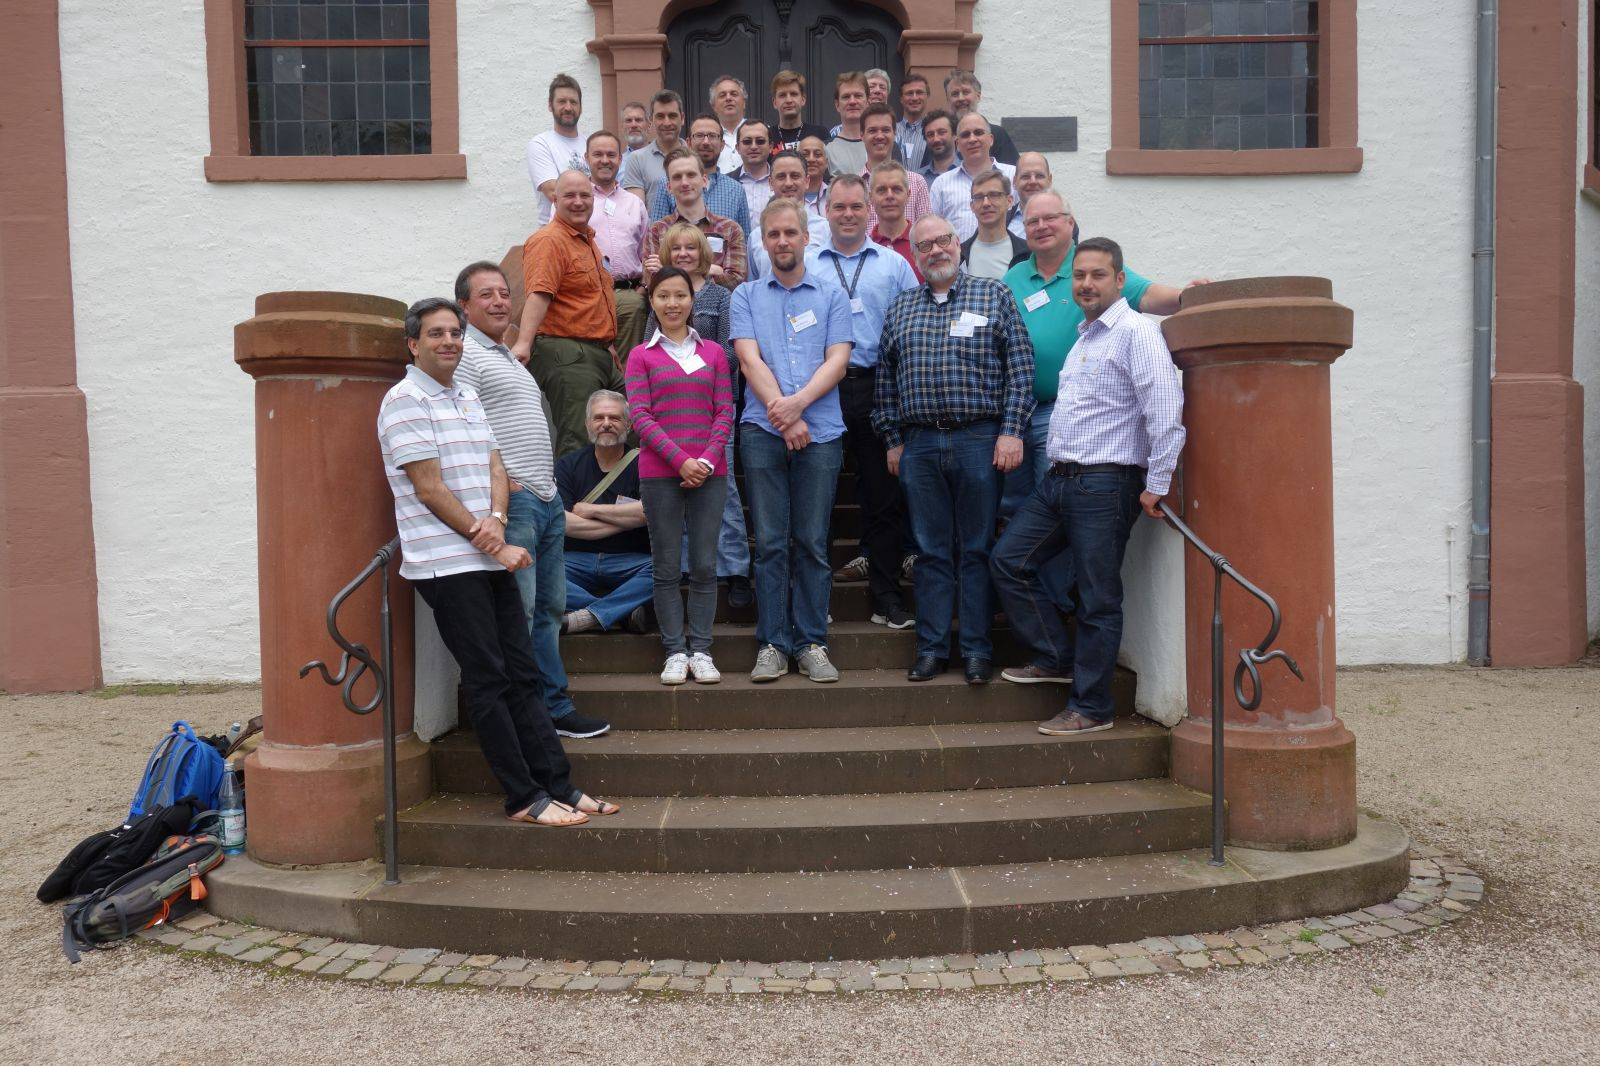
\includegraphics[width=1.0\textwidth]{16251.jpg}
\end{center}

\end{document}
